\documentclass{beamer}

\usetheme{Darmstadt}
\usefonttheme[onlylarge]{structurebold}
\setbeamerfont*{frametitle}{size=\normalsize,series=\bfseries}
\setbeamertemplate{navigation symbols}{}

% Standard packages

\usepackage[english]{babel}
\usepackage[latin1]{inputenc}
\usepackage{times}
\usepackage[T1]{fontenc}
\usepackage{float}
\usepackage{graphicx}
\usepackage{subcaption}
\usepackage{ifthen}
\usepackage{minted}
\usepackage{verbatim}
%\usepackage{multimedia}
\usepackage{movie15}

% Setup TikZ
\usepackage{tikz}
\usetikzlibrary{arrows}
\tikzstyle{block}=[draw opacity=0.7,line width=1.4cm]


% Author, Title, etc.
\title[Pure Functional Epidemics] 
{%
  Pure Functional Epidemics \\ An Agent-Based Approach%
}

\author[Thaler, Altenkirch, Siebers]
{
  Jonathan~Thaler \and
  Thorsten~Altenkirch \and
  Peer-Olaf~Siebers
}

\institute[University of Nottingham, United Kingdom]
{
  University of Nottingham, United Kingdom
}

\date[Implementation and Application of Functional Languages (IFL) 2018]
{IFL 2018}

% The main document
\begin{document}

\begin{frame}
  \titlepage
\end{frame}

\section{Introduction}
\begin{frame}{Research Questions}
\begin{itemize}
  \item \textbf{How} can we implement Agent-Based Simulation in (pure) functional programming e.g. Haskell?
  \item \textbf{What} are the benefits and drawbacks?
\end{itemize}
\end{frame}

\begin{frame}{Agent-Based Simulation (ABS)} 
  \begin{block}{Example}
    \textit{\textbf{Simulate} the spread of an infectious disease in a city. \\ What are the \textbf{dynamics} (peak, duration of disease)?}
  \end{block}
  
  \begin{enumerate}
    \item Start with population \, \, \, \, \, \, \, $\to$ Agents
 	\item Situated in City \, \, \, \, \, \, \, \, \, \, \, \,\, $\to$ Environment
 	\item Interacting with each other \, $\to$ local interactions
 	\item Creating dynamics \, \, \, \, \, \, \, \,\,\, $\to$ emergent system behaviour
 	\item Therefore ABS \, \, \, \, \, \, \, \, \, \, \, \,\,\, $\to$ bottom-up approach
  \end{enumerate}
\end{frame}

\begin{frame}{SIR Model}
  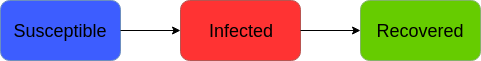
\includegraphics[width=0.7\textwidth]{./fig/SIR_transitions.png}
  
  \begin{itemize}
    \item Population size $N = 1,000$
 	\item Contact rate $\beta = 0.2$
 	\item Infection probability $\gamma = 0.05$
 	\item Illness duration $\delta = 15$
 	\item 1 initially infected agent
  \end{itemize}
    
  \begin{block}{System Dynamics}
    Top-Down, formalised using Differential Equations, give rise to dynamics.
  \end{block}
\end{frame}

\begin{frame}{SIR Model Dynamics}
  \center
  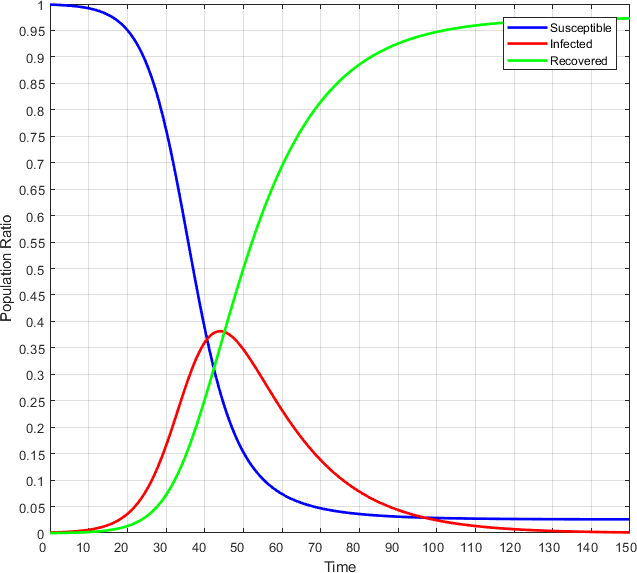
\includegraphics[width=0.7\textwidth]{./fig/SIR_SD_001dt.png}
\end{frame}

\begin{frame}{How to implement ABS?}
  \begin{block}{Established, state-of-the-art approach in ABS}
	Object-Oriented Programming in Python, Java,...
  \end{block}
  
  \begin{block}{We want (pure) functional programming}
	Purity, explicit about side-effects, declarative, reasoning, parallelism, concurrency, property-based testing,...
  \end{block}
  
  \begin{block}{How can we do it?}
  	Functional Reactive Programming
  \end{block}
\end{frame}

\begin{frame}{Functional Reactive Programming (FRP)}
  \begin{itemize}
    \item Continuous- \& discrete-time systems in FP
 	\item Signal Function 
 	\item Events
 	\item Random-number streams
 	%\item Running signal-functions in pure way
 	\item \textit{Arrowized} FRP using the \textit{Yampa} library
  \end{itemize}
\end{frame}

\begin{frame}{Signal Function (SF)}
  \begin{block}{Process over time}
  \begin{flalign*}
	SF \, \alpha \, \beta \approx Signal \, \alpha \rightarrow Signal \, \beta \\
	Signal \, \alpha \approx Time \rightarrow \alpha 
  \end{flalign*}
  \end{block}
  
  \begin{block}{Agents as Signal Functions}
  \begin{itemize}
  	\item Clean interface (input / output)
  	\item Pro-activity by perceiving time
  \end{itemize}
  \end{block}
\end{frame}

\begin{frame}[fragile]{FRP combinators}
\begin{block}{Dynamic change of behaviour}
\begin{minted}[fontsize=\tiny]{haskell}
switch :: SF inp (out, Event e) -> (e -> SF inp out) -> SF inp out
\end{minted}
\end{block}

\begin{block}{Stochastic event source}
\begin{minted}[fontsize=\tiny]{haskell}
occasionally :: RandomGen g => g -> Time -> b -> SF a (Event b)
\end{minted}
\end{block}

\begin{block}{Deterministic event source}
\begin{minted}[fontsize=\tiny]{haskell}
after :: Time -> b -> SF a (Event b)
\end{minted}
\end{block}

\begin{block}{Random number stream}
\begin{minted}[fontsize=\tiny]{haskell}
noiseR :: (RandomGen g, Random b) => (b, b) -> g -> SF a b
\end{minted}
\end{block}

\begin{block}{Infinitesimal delay (1 step)}
\begin{minted}[fontsize=\tiny]{haskell}
iPre :: a -> SF a a
\end{minted}
\end{block}
\end{frame}

%\begin{frame}[fragile]{FRP combinators}
%\begin{block}{Dynamic change of behaviour}
%\begin{minted}[fontsize=\tiny]{haskell}
%switch :: SF in (out, Event t) -> (t -> SF in out) -> SF in out
%\end{minted}
%\end{block}
%
%\center
%  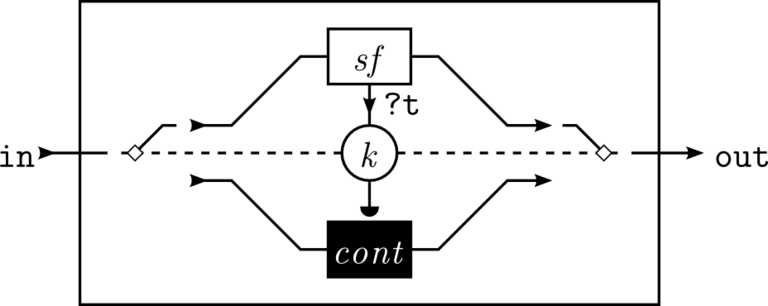
\includegraphics[width=0.7\textwidth]{./fig/yampa_switch.png}
%\end{frame}

%\begin{frame}[fragile]{Switch}
%  \center
%  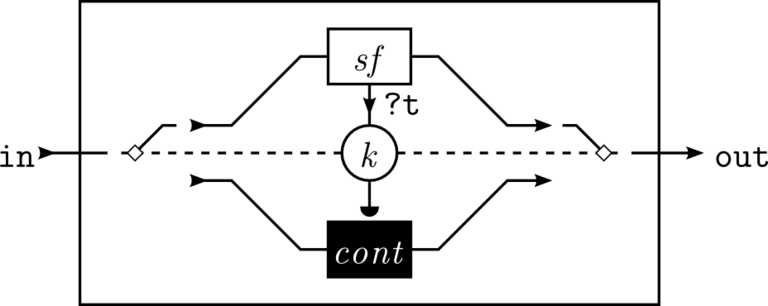
\includegraphics[width=0.7\textwidth]{./fig/yampa_switch.png}
%
%\begin{minted}[fontsize=\tiny]{haskell}
%switch :: SF in (out, Event t) -> (t -> SF in out) -> SF in out
%\end{minted}
%\end{frame}

\section{Agent-Based SIR in Haskell}
\begin{frame}{Update Semantics}
  %TODO: sequential is wrong semantics because all agents act at the sa.e time, if we impose an ordering it could be the case that e.g. the infection spreads from top left corner to bottom right but not the other way round. for many ab models which run sequentially the established approach is thus to shuffle the agents in each step to avoid these kind of semantic problems. In FP we can enforce such an iteation strategy already in the types. the flaw reflects exactly my iterating paper message: the strategy needs to reflect the semantics of the model

%TODO: make clear that ABS often runs agents sequentially and shuffles them. there is no agreed "true" way as we have shown as itvresults in different semantics but in  functional programming the parallel approach is the best fit. and for SIR its the only correct one

\hspace*{1cm}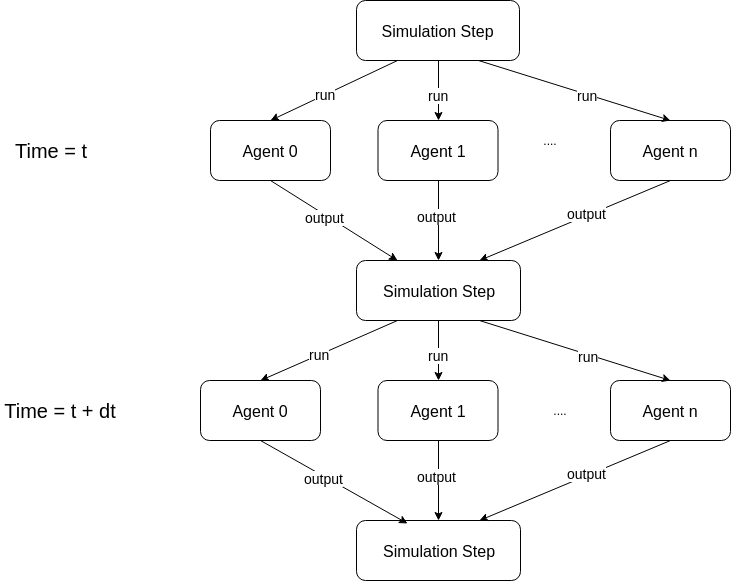
\includegraphics[width=0.7\textwidth]{./fig/parallel_strategy.png}\hspace*{-1cm}
\end{frame}

\begin{frame}{Arrowized Programming}
\begin{block}{Monads}
\texttt{\textbf{do} \\
\hspace{\parindent} \, out1 $\leftarrow$ \textit{comp1} \\
\hspace{\parindent} \, out2 $\leftarrow$ \textit{comp2 out1} \\
\hspace{\parindent} \, return out2}
\end{block}
	
\begin{block}{Arrows}
\texttt{\textbf{proc} input \textbf{do} \\
\hspace{\parindent} \, out1 $\leftarrow$ \textit{comp1} $\prec$ input \\
\hspace{\parindent} \, out2 $\leftarrow$ \textit{comp2} $\prec$ out1 \\
\hspace{\parindent} \, returnA $\prec$ out2}
\end{block}
\end{frame}

\begin{frame}[fragile]{Some Types...}
\begin{minted}[fontsize=\footnotesize, linenos]{haskell}
data SIRState = Susceptible | Infected | Recovered

type SIRAgent = SF [SIRState] SIRState 
  
sirAgent :: RandomGen g => g -> SIRState -> SIRAgent
sirAgent g Susceptible = susceptibleAgent g
sirAgent g Infected    = infectedAgent g
sirAgent _ Recovered   = recoveredAgent

recoveredAgent :: SIRAgent
recoveredAgent = arr (const Recovered)
\end{minted}
\end{frame}

\begin{frame}[fragile]{Susceptible Agent}
\begin{minted}[fontsize=\tiny, linenos]{haskell}
susceptibleAgent :: RandomGen g => g -> SIRAgent
susceptibleAgent g 
    = switch 
      -- delay switching by 1 step to prevent against transition
      -- from Susceptible to Recovered within one time-step
      (susceptible g >>> iPre (Susceptible, NoEvent)) 
      (const (infectedAgent g))
  where
    susceptible :: RandomGen g => g -> SF [SIRState] (SIRState, Event ())
    susceptible g = proc as -> do
      -- generate an event on average with given rate
      makeContact <- occasionally g (1 / contactRate) () -< ()
      if isEvent makeContact
        then (do
          -- draw random contact
          a <- drawRandomElemSF g -< as
          case a of
            -- contact with infected => get infected with prob.
            Infected -> do
              -- returns True with given probability
              i <- randomBoolSF g infectivity -< ()
              if i
                -- got infected => infection event => transition to infected
                then returnA -< (Infected, Event ())
                else returnA -< (Susceptible, NoEvent)
             _       -> returnA -< (Susceptible, NoEvent))
        else returnA -< (Susceptible, NoEvent)
\end{minted}
\end{frame}

\begin{frame}{Dynamics $\Delta t = 0.1$}
\begin{figure}
\begin{center}
	\begin{tabular}{c c}
		\begin{subfigure}[b]{0.4\textwidth}
			\centering
			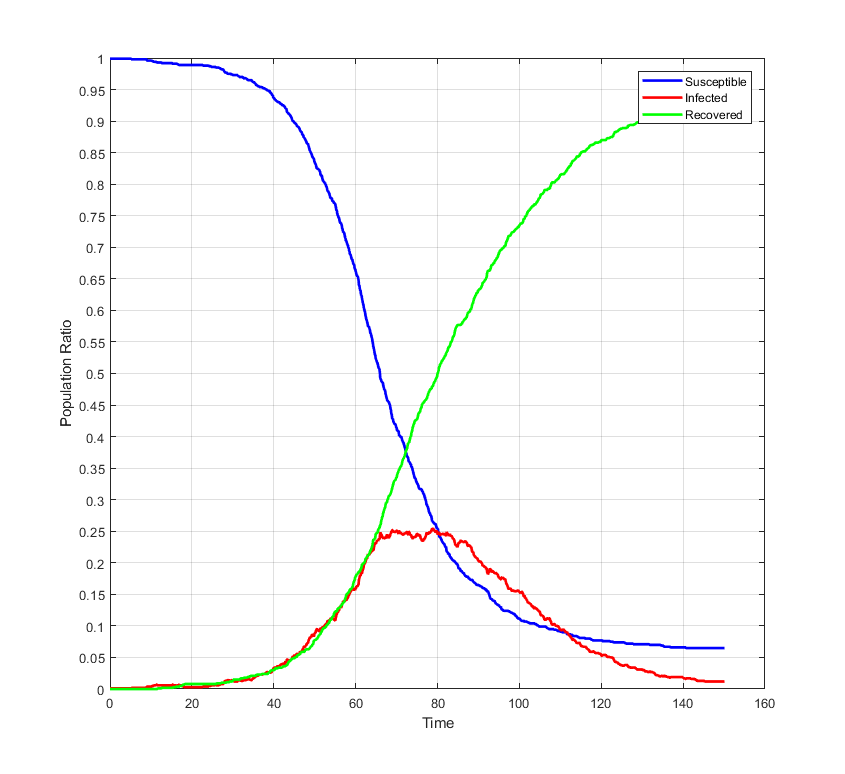
\includegraphics[width=0.95\textwidth, angle=0]{./fig/SIR_Yampa_dt01.png}
			\caption{Agent-Based approach}
		\end{subfigure}
    	
    	&
  
		\begin{subfigure}[b]{0.4\textwidth}
			\centering
			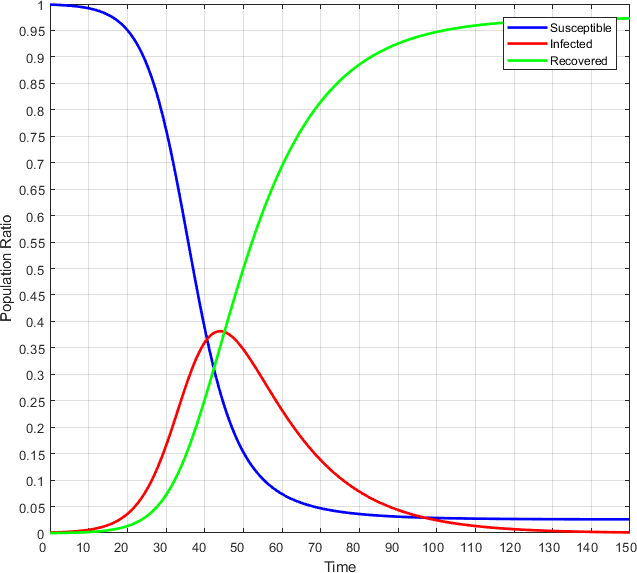
\includegraphics[width=1\textwidth, angle=0]{./fig/SIR_SD_001dt.png}
			\caption{System Dynamics}
		\end{subfigure}
	\end{tabular}
\end{center}
\end{figure}
\end{frame}

\begin{frame}{Dynamics $\Delta t = 0.01$}
\begin{figure}
\begin{center}
	\begin{tabular}{c c}
		\begin{subfigure}[b]{0.4\textwidth}
			\centering
			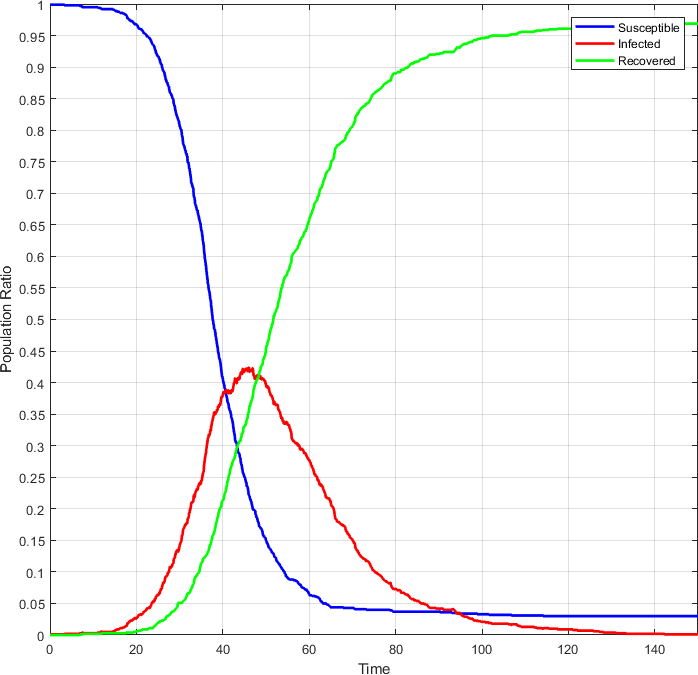
\includegraphics[width=0.95\textwidth, angle=0]{./fig/SIR_Yampa_dt001.png}
			\caption{Agent-Based approach}
		\end{subfigure}
    	
    	&
  
		\begin{subfigure}[b]{0.4\textwidth}
			\centering
			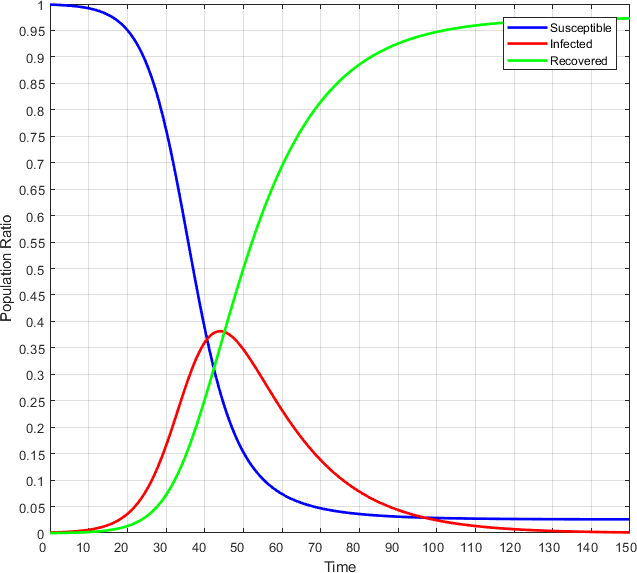
\includegraphics[width=1\textwidth, angle=0]{./fig/SIR_SD_001dt.png}
			\caption{System Dynamics}
		\end{subfigure}
	\end{tabular}
\end{center}
\end{figure}
\end{frame}

\begin{frame}{Reflection}
  \begin{block}{So far...}
  \begin{itemize}
    \item Agents with stochastic behaviour %- implemented as an individual, behaviour depending on internal state.
	\item Time \& Feedback % - simulation over virtual time, modelled explicitly, divided into \textit{fixed} $\Delta t$, at each step all agents executed.
	%\item Feedback %- output state of agent in time-step $t$ is input for next time-step $t + \Delta t$.
	%\item \textbf{Environment} - fully-connected network (complete graph).
	\item Deterministic dynamics %- repeated runs with same initial random-number generator result in same dynamics.
	\item Parallel, lock-step semantics
  \end{itemize}
  \end{block}
    
  \begin{block}{Whats next?}
    \begin{itemize}
  	  \item Problem - correlated random numbers
	  \item Spatiality - structured environment
	\end{itemize}
  \end{block}
\end{frame}

\section{Solving Random Number Correlation}
\begin{frame}{Solving Random Number Correlation}
  \begin{block}{Elegant Approach}
  	\textit{Random Monad}
  \end{block} 
  
  \begin{block}{Problem}
  	\textit{Yampa} not monadic
  \end{block}
  
  \begin{block}{Solution}
    Monadic Stream Functions 
  \end{block}
\end{frame}

\begin{frame}[fragile]{Monadic Stream Functions (MSFs)}
\begin{block}{Concept}
\begin{itemize}
  \item Signal Functions + monadic context 
  \item \textit{Dunai} - Perez et al 
  \item \textit{BearRiver} - \textit{Yampa} built on top of \textit{Dunai}
\end{itemize}
\end{block}

\begin{block}{Definition}
\begin{minted}[fontsize=\tiny]{haskell}
newtype MSF m a b = MSF {unMSF :: MSF m a b -> a -> m (b, MSF m a b)}

arrM :: Monad m -> (a -> m b) -> MSF m a b
arrM_ :: Monad m -> m b -> MSF m a b
\end{minted}
\end{block}
    
\begin{block}{Monadic Stochastic Event Source}
\begin{minted}[fontsize=\tiny]{haskell}
occasionallyM :: MonadRandom m => Time -> b -> SF m a (Event b)
\end{minted}
\end{block}

\begin{block}{Monadic Agent Signal Function}
\begin{minted}[fontsize=\tiny]{haskell}
type SIRAgent g = SF (Rand g) [SIRState] SIRState 
\end{minted}
\end{block}
\end{frame}

\section{Adding Spatiality}
\begin{frame}[fragile]{Defining Spatiality}
\begin{figure}
\begin{center}

\includegraphics[width=0.2\textwidth]{./fig/moore.png}
\caption*{Moore Neighbourhood}
\end{center}
\end{figure}

\begin{block}{Some types...}
\begin{minted}[fontsize=\tiny]{haskell}
type Disc2dCoord = (Int, Int)
type SIREnv      = Array Disc2dCoord SIRState

type SIRAgent g  = SF (Rand g) SIREnv SIRState
\end{minted}
\end{block}
\end{frame}

\begin{frame}{Spatial Dynamics}
\begin{figure}
\begin{center}
	\begin{tabular}{c c}
		\begin{subfigure}[b]{0.4\textwidth}
			\centering
			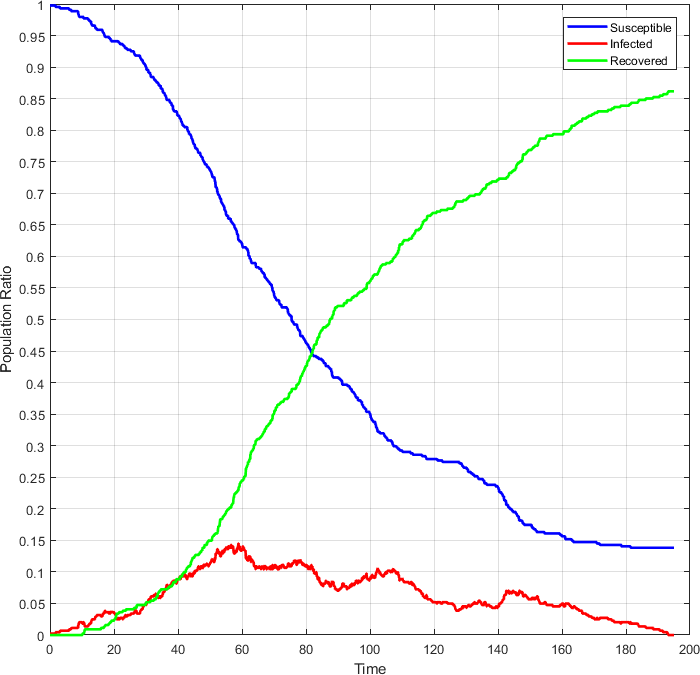
\includegraphics[width=0.95\textwidth, angle=0]{./fig/SIR_Dunai_dt001.png}
			\caption{Agent-Based}
		\end{subfigure}
    	
    	&
  
		\begin{subfigure}[b]{0.4\textwidth}
			\centering
			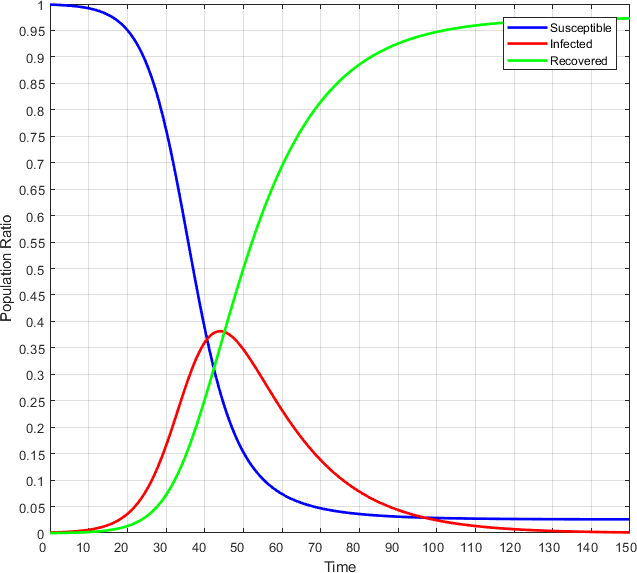
\includegraphics[width=1\textwidth, angle=0]{./fig/SIR_SD_001dt.png}
			\caption{System Dynamics}
		\end{subfigure}
	\end{tabular}
\end{center}
\end{figure}
\end{frame}

\begin{frame}{Spatial Visualisation}
%\movie[width=10cm,height=5.5cm]{Dynamics 21x21 2D Environment}{./video/SIR_DUNAI_dt001.mp4}
\includemovie[rate=2]{11cm}{6.5cm}{./video/SIR_DUNAI_dt001.mp4}
\end{frame}

\section{Discussion}
%\begin{frame}{Performance}
%  \begin{block}{Experiment}
%    Spatial Agent-Based SIR, 51x51 Grid (2,601 agents), $t = 100$, $\Delta t = 0.1$, avg. 8 runs
%  \end{block}
%  
%  \begin{block}{Haskell}
%  	72.5 sec
%  \end{block}
%  
%  \begin{block}{RePast ($\Delta t = ?$)}
%  	10.8 sec
%  \end{block}
%  
%  \begin{block}{STM Haskell}
%  	8.6 sec on Amazon S2, 16 cores (other paper)
%  \end{block}
%\end{frame}

\begin{frame}{Conclusion}
  \begin{itemize}
    \item Purity guarantees reproducibility at compile time
    \item Enforce and guarantee update semantics at compile time
    \item Performance :(
    \item Agent-Identity a bit lost
    \item Agent-Interaction is main difficulty
  \end{itemize}
\end{frame}

\begin{frame}{}
  \begin{center}
  Thank You!
  \end{center}
\end{frame}
\end{document}